% --- ARCHIVO: Cap5_Analisis_Informes/analisis_informes.tex ---

\chapter{Análisis de Informes e Interpretaciones de los Agentes}
\label{cap:analisis_informes}

\section{La visión del Gobierno y el Operador del Sistema (REE): seguridad nacional, cumplimiento normativo y causalidad multifactorial}
\label{sec:vision_gobierno}

\lettrine[lines=3, lhang=0.1]{E}{l} escrutinio de la documentación oficial emitida tras el colapso del 28 de
abril revela una arquitectura argumental de naturaleza institucional,
vertebrada a través del Informe del Comité de Análisis gubernamental y el
dictamen técnico de Red Eléctrica de España (REE). La narrativa de la
Administración tipifica el apagón no como un error de diseño en la topología
de control ni como consecuencia directa de las maniobras operativas, sino
como un evento de naturaleza multifactorial: una convergencia de
\textit{demanda valle}, penetración masiva de \textit{Recursos Basados en
Inversores} (IBR) y comportamiento técnico inadecuado de los agentes
privados que, actuando de forma simultánea, superó los umbrales contemplados
por el \textit{Criterio $N-1$}\textsuperscript{\ref{anexo:criterio_n1}}
\cite{gobierno2025,ree2025}.

La defensa técnica esgrimida por Red Eléctrica aborda la decisión de
\textit{mallar} la red de transporte en los instantes previos al
\textit{cero de tensión} como una medida paliativa estrictamente
protocolizada frente a las oscilaciones registradas. Según la tesis oficial,
la red operaba en un estado de régimen permanente normalizado hasta la
irrupción de una \textit{oscilación forzada} atípica de 0,6~Hz, cuyo origen
el operador atribuye ---como hipótesis compatible con los datos
disponibles--- al lazo de control de una planta solar fotovoltaica en la
provincia de Badajoz. Para amortiguar tanto esta perturbación como el
posterior \textit{modo inter-área} de 0,2~Hz, REE sostiene que el
acoplamiento de líneas y reactancias constituía la vía canónica de
actuación, reconociendo el incremento tensional como un efecto secundario
indeseado, pero no como el factor primario del colapso
\cite{gobierno2025,ree2025}.

La secuencia cronológica oficial de estas fases se ilustra en la
figura~\ref{fig:cronograma_fases}
(p.~\pageref{fig:cronograma_fases}) del
capítulo~\ref{cap:reaccion_reposicion}.

El argumento central del informe gubernamental traslada la responsabilidad
material del desastre al comportamiento del parque generador privado,
sosteniendo que la red disponía de capacidad termodinámica y topológica
para absorber el transitorio del \textit{mallado} si los agentes hubiesen
operado conforme a la normativa vigente. El análisis oficial documenta
que aproximadamente el 22~\% de las instalaciones del \textit{Régimen
de Renovables, Cogeneración y Residuos}
(RCR)\textsuperscript{\ref{anexo:rcr}} analizadas no cumplían el criterio
de factor de potencia exigido por el RD~413/2014 en el momento crítico.
No obstante, el propio informe matiza que este incumplimiento podría
atribuirse, al menos parcialmente, al efecto capacitivo de las
infraestructuras de evacuación cuando operan con baja generación,
reconociendo así que la frontera entre incumplimiento normativo y
limitación técnica estructural no es nítida. Según REE, al no absorber
\textit{potencia reactiva} inductiva en los minutos más críticos, estas
instalaciones privaron al sistema del margen necesario para contener la
escalada de tensión \cite{gobierno2025,ree2025}.

Esta imputación de insuficiencia técnica no se restringe a las tecnologías
asíncronas. El informe gubernamental señala a las instalaciones de
generación convencional sujetas al \textit{Procedimiento de Operación
7.4} (P.O.~7.4)\textsuperscript{\ref{anexo:po74}} ---ciclos combinados de
gas y parque nuclear--- por no haber respondido con la absorción de
potencia reactiva exigida. De forma particular, se documenta el caso de
una central térmica en la zona sur que, en lugar de drenar energía
reactiva de la red para mitigar la sobretensión, operó inyectando
potencia reactiva capacitiva adicional al sistema. La conclusión de la
Administración es que el colapso habría podido evitarse si el conjunto
de generadores hubiese garantizado un soporte de reactiva continuo,
dejando al Operador del Sistema sin los recursos dinámicos necesarios
para contener el transitorio \cite{gobierno2025,ree2025}.

\begin{figure}[H]
\centering
\begin{tikzpicture}[
    node distance=1.8cm and 1.2cm,
    box/.style={rectangle, rounded corners=4pt, draw, minimum width=3.6cm,
                minimum height=1.1cm, align=center, font=\small},
    root/.style={box, fill=blue!10, draw=blue!50},
    leftbox/.style={box, fill=violet!10, draw=violet!40},
    midbox/.style={box, fill=teal!10, draw=teal!40},
    rightbox/.style={box, fill=orange!10, draw=orange!40},
    arr/.style={->, thick, gray!70}
]

\node[root] (origen) {\textbf{Origen multifactorial}};

\node[leftbox,  below left=1.8cm and 1.6cm of origen]
    (tension) {\textbf{Control de tensión}\\\textbf{insuficiente}\\{\footnotesize (P.O.~7.4)}};

\node[midbox,   below=1.8cm of origen]
    (oscilaciones) {\textbf{Oscilaciones}\\{\footnotesize condicionan el sistema}};

\node[rightbox, below right=1.8cm and 1.6cm of origen]
    (desconexiones) {\textbf{Desconexiones}\\{\footnotesize de generación}\\{\footnotesize (algunas prematuras)}\\{\footnotesize $\rightarrow$ sobretensión}};

\draw[arr] (origen) -- (tension);
\draw[arr] (origen) -- (oscilaciones);
\draw[arr] (origen) -- (desconexiones);

\end{tikzpicture}
\caption[Origen multifactorial del colapso según el Comité de Análisis.]{%
Esquema de causalidad multifactorial del colapso según el Comité de
Análisis del Gobierno. Fuente: Comité de Análisis del Gobierno
\cite{gobierno2025}}
\label{fig:origen_multifactorial}
\end{figure}

La figura~\ref{fig:origen_multifactorial} resume la estructura causal
articulada por la Administración: el control de tensión calificado como
insuficiente conforme al P.O.~7.4, las oscilaciones electromecánicas como
condicionantes del sistema, y las desconexiones de generación ---algunas
de ellas calificadas como prematuras por el operador--- como vector
final de la sobretensión. La presentación oficial subraya, dentro de
este esquema, el incumplimiento técnico de los generadores como factor
material de la cascada.

La magnitud material del evento ---paralización de infraestructuras
críticas, paradas de emergencia en refinerías y colapso de las redes de
telecomunicaciones--- proporcionó el contexto para que el Gobierno
elevara el apagón a una cuestión de seguridad nacional. El suceso motivó
la constitución de un Comité avalado por el Consejo de Seguridad Nacional
(CSN) y la declaración oficial de ``Crisis de Electricidad'' ante la
Comisión Europea, amparándose en el Reglamento (UE)~2019/941. Este
encuadre institucional tuvo consecuencias operativas directas: justificó
la suspensión de los mecanismos de mercado durante la Fase~4 y otorgó a
REE autoridad plena para despachar a los generadores bajo criterios
exclusivamente técnicos, marginando el \textit{Orden de Mérito} económico
\cite{gobierno2025,entsoe2025}.

\vspace{0.6cm}
\begin{figure}[H]
    \centering
    
\includegraphics[width=0.85\textwidth]{figuras/portada_informe_csn.png}
    \vspace{0.2cm}
    \caption[Portada del informe oficial con los logotipos institucionales.]{%
    Portada del informe oficial del Comité de Análisis con los logotipos
    institucionales. Fuente: Gobierno de España \cite{gobierno2025}}
    \label{fig:portada_informe_csn}
\end{figure}
\vspace{0.6cm}

La participación directa del Consejo de Seguridad Nacional en la
elaboración del informe (figura~\ref{fig:portada_informe_csn}) refleja
el rango institucional con el que el Gobierno abordó el apagón: no como
un fallo técnico circunscrito a la red de transporte, sino como un
incidente con implicaciones para la seguridad de las infraestructuras
críticas del Estado.

Desde una perspectiva analítica, la narrativa gubernamental presenta una
coherencia interna apreciable: identifica incumplimientos normativos
documentados, apunta a un comportamiento técnico anómalo verificable en
al menos una central síncrona, y sostiene que las maniobras del operador
fueron protocolizadas. Sin embargo, como se desarrolla en la
sección~\ref{sec:vision_icai} (p.~\pageref{sec:vision_icai}), esta
postura no responde a los argumentos periciales sobre la magnitud de la
reactiva capacitiva inyectada por el \textit{mallado} ni sobre la
inobservabilidad del operador en la red de 220~kV por el fenómeno de
\textit{Tap-Lag}: dos elementos que, según el informe ICAI, habrían
hecho inevitable el colapso con independencia del nivel de cumplimiento
normativo de los generadores \cite{icai2025}.

\clearpage
% --------------------------------------------------------------
\section{La visión de Redeia: defensa de la operación del sistema y análisis de la respuesta técnica de los generadores}
\label{sec:vision_redeia}
% --------------------------------------------------------------

La posición técnica adoptada por Red Eléctrica de España (Redeia) tras el
apagón se articula en torno a la defensa de sus decisiones operativas en
el despacho central, trasladando la génesis del colapso hacia un fallo
generalizado en el comportamiento técnico del parque de generación. El
operador sostiene que, hasta el instante en que comenzaron las
perturbaciones dinámicas externas, la red de transporte operaba en
estricta normalidad, cumpliendo los márgenes del P.O.~1.1 y garantizando
el Criterio $N-1$. Según esta narrativa, el sistema se vio sometido a un
estrés electromecánico severo e imprevisto: primero, por la irrupción de
una oscilación forzada de 0,6~Hz, cuyo origen el operador correlaciona
con la operación de una instalación fotovoltaica en la provincia de
Badajoz; y escasos minutos después, por un modo inter-área natural de
0,2~Hz \cite{ree2025}.

Frente a la crítica del sector generador sobre el \textit{mallado} de la
red, Redeia ofrece una justificación técnica y procedimental que conviene
examinar con precisión. El informe de REE subraya un aspecto que, con
frecuencia, se omite en las críticas: las oscilaciones iniciales no
provocaron sobretensiones sino caídas de tensión en los nudos de la red
de transporte. Ante este riesgo de inestabilidad, el Centro de Control
ejecutó una batería de acciones estrictamente protocolizadas: la
reconexión de circuitos para robustecer la topología, el acoplamiento de
reactancias y la coordinación con el operador francés (RTE) para conmutar
el enlace \textit{HVDC} al modo de potencia constante (PMODE1). El propio
informe reconoce que estas maniobras ``contribuyeron al alza en las
tensiones'' y supusieron ``una configuración distinta del sistema de
la prevista al inicio del día'', aunque las califica como medidas
necesarias para contener las oscilaciones. REE defiende que cualquier
incremento tensional posterior hubiera sido absorbible por el sistema si los
agentes hubiesen cumplido con sus obligaciones normativas \cite{ree2025}.

\vspace{0.6cm}
\begin{figure}[H]
    \centering
    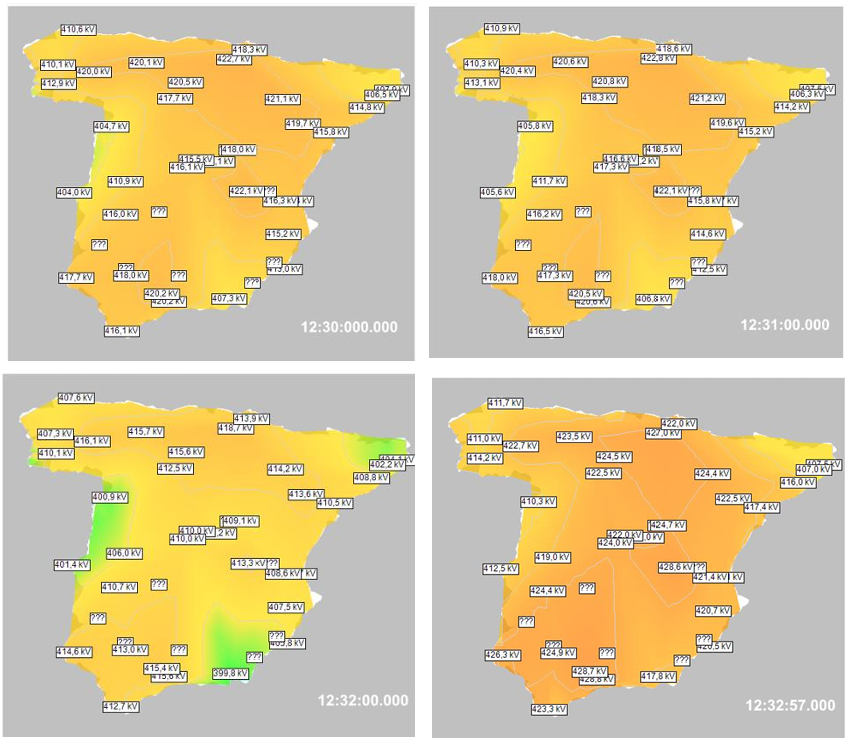
\includegraphics[width=0.85\textwidth]{figuras/mapas_termicos_tension_ree.png}
    \vspace{0.2cm}
    \caption[Mapas térmicos de tensión en la red de 400 kV, según REE (12:30--12:32:57).]{%
    Mapas térmicos de tensión en la red de transporte de 400~kV en los
    instantes previos al disparo raíz (12:30--12:32:57~CEST) según el
    análisis del Operador del Sistema. Fuente: Informe de Red Eléctrica
    \cite{ree2025}}
    \label{fig:mapas_termicos_ree}
\end{figure}
\vspace{0.6cm}

La figura~\ref{fig:mapas_termicos_ree} reproduce la cartografía oficial
del Operador del Sistema durante los minutos previos al colapso. Sobre
esta base, REE sostiene que ---a pesar de las maniobras de
\textit{mallado}--- los perfiles de tensión registrados en la red de
400~kV se mantuvieron dentro de los rangos operativos definidos en el
P.O.~1.1 hasta el inicio de las desconexiones masivas en las redes
colectoras subyacentes.

El núcleo del dictamen forense de Redeia es un escrutinio de la respuesta
técnica del parque generador. La crítica más documentada se dirige hacia
las instalaciones de generación síncrona convencional sujetas al
P.O.~7.4 ---ciclos combinados y nuclear---, que están obligadas a
proporcionar control de tensión por consigna. El informe constata que,
prácticamente, la totalidad de los grupos acoplados en las zonas centro y
sur no absorbieron toda la potencia reactiva necesaria en uno o varios
períodos de la mañana del 28 de abril. En particular, una central de la
zona sur mostró un comportamiento visiblemente distinto al del resto: su
absorción de reactiva no presentó relación con el perfil de tensión, e
incluso inyectó reactiva capacitiva en lugar de absorberla, contribuyendo
a agravar la sobretensión. REE atribuye esta respuesta insuficiente a la
operación de estos grupos dentro de ``bandas muertas'' normativas, lo que
retrasó su actuación hasta que la desviación de tensión ya era
significativa \cite{ree2025}.

Esta imputación se extiende a los \textit{Recursos Basados en Inversores}
(IBR) del régimen RCR. Aunque Redeia reconoce que estas instalaciones no
estaban obligadas a control dinámico de tensión bajo la normativa
vigente, sí tenían el deber legal de cumplir los valores de factor de
potencia consignados conforme al RD~413/2014. El análisis del operador
sobre las 850 instalaciones de mayor generación en ese momento documenta
que cerca del 22~\% no cumplían el criterio de factor de potencia
exigible, si bien el propio informe matiza que parte de este
incumplimiento podría atribuirse al efecto capacitivo de las
infraestructuras de evacuación cuando operan con baja generación. Para
el operador, la inhibición en la absorción de reactiva por parte del
parque renovable transformó la red en un entorno con capacidad reducida
para amortiguar la inyección capacitiva de las líneas en vacío
\cite{ree2025}.

Para culminar su argumentación, Redeia aborda la naturaleza de los
disparos que iniciaron la cascada. La postura oficial califica algunas
de estas desconexiones como ``no ajustadas'' o producidas ``antes de
tiempo'': el operador señala que, en el lado de 400~kV, la tensión en el
nudo de Granada se encontraba en 418~kV en el instante previo al disparo
raíz, dentro de los límites normativos, por lo que las instalaciones
``no deberían haberse desconectado'' según su lectura de la red de
transporte. Esta calificación choca directamente con la tesis del sector
generador, que argumenta que las protecciones actuaron ante tensiones
reales de 242,5~kV en el lado de 220~kV del autotransformador
---provocadas por el \textit{Tap-Lag}---, y la declaración del propio titular de la
infraestructura quien confirmó que la protección ``estaba correctamente
ajustada y funcionó adecuadamente''. La resolución de esta contradicción
es el eje central de la disputa forense entre ambas partes, como se
analiza en la sección~\ref{sec:vision_icai}
(p.~\pageref{sec:vision_icai}) \cite{icai2025,ree2025}.

Finalmente, Redeia aborda explícitamente el papel de la \textit{inercia
del sistema} en el colapso, descartando que fuese su causa material. El
informe documenta que la inercia disponible el 28 de abril era de
$H = 2,3$~s, por encima del umbral de 2~s recomendado por ENTSO-E, y
concluye que, incluso con mayor inercia, ``la ola de sobretensión hubiera
provocado el efecto cascada en todo caso'' ya que las condiciones de
sobretensión persistieron hasta las 12:33:23~CEST, independientemente de
la frecuencia. Para el operador, la pérdida de sincronismo fue el
resultado de un parque generador que no reguló su tensión de forma
adecuada, eximiendo así a las maniobras del despacho central de
responsabilidad material en el desencadenamiento del colapso
\cite{ree2025}.


\begin{table}[H]
\centering
\caption[Secuencia de factores desencadenantes del colapso según Red Eléctrica.]{%
Secuencia oficial de factores desencadenantes del colapso según Red
Eléctrica (Redeia). Los eventos marcados como ``disparo inadecuado''
constituyen el eje central de la controversia con el sector generador,
que los califica como actuaciones de autoprotección normativa ante
\textit{Tap-Lag}. Fuente: Elaboración propia}
\label{tab:decalogo_ree}
\vspace{0.3cm}
\small
\begin{tabularx}{\textwidth}{>{\centering\bfseries}p{1.1cm} >{\centering\bfseries}p{1.3cm} >{\centering\arraybackslash}X}
\toprule
\textbf{Evento} & \textbf{Referencia} & \textbf{Descripción} \\
\midrule

1 & N-1 &
Oscilación forzada de 0,6~Hz con posible origen en una planta
fotovoltaica de Badajoz. Activación de medidas protocolizadas: maniobra
de reactancias, acoplamiento de líneas y cambios de programas. \\
\addlinespace

2 & N-2 &
Oscilación natural inter-área de 0,2~Hz. Nuevas maniobras de
amortiguamiento: reconexión de líneas y ajuste de programas de
intercambio. \\
\addlinespace

3 & N-3 &
La generación sujeta al P.O.~7.4 no absorbe la potencia reactiva
requerida por consigna. \\
\addlinespace

4 & N-4 &
Las variaciones de generación RCR afectan al control de tensión. Un
porcentaje significativo de plantas incumple sus obligaciones de factor
de potencia. \\
\addlinespace

5 & --- &
La generación convencional solicitada tras las oscilaciones no llega a
acoplarse. \\
\addlinespace

6 & N-5 &
Pérdidas de generación distribuida ($<\!1$~MW) y autoconsumo (435~MW)
antes de las 12:32:57~CEST. \\
\addlinespace

7 & N-6 &
\textbf{Disparo del transformador de evacuación en Granada} a las
12:32:57~CEST. REE registra 418~kV en el lado de 400~kV, dentro de
límites normativos. \\
\addlinespace

8 & N-7 &
Disparo de generación termosolar y fotovoltaica en Badajoz sin
información en el punto frontera con la red de transporte. \\
\addlinespace

9 & N-8 &
Disparo de planta fotovoltaica en Badajoz en subestación distinta,
también sin visibilidad en frontera. \\
\addlinespace

10 & --- &
Disparo de 3 parques eólicos en Segovia sin información en el punto
frontera con la red de transporte. \\
\addlinespace

11 & --- &
Disparo de parque eólico y planta fotovoltaica en Huelva sin información
en frontera. \\
\addlinespace

12 & N-9 &
Disparos de plantas fotovoltaicas en la provincia de Sevilla. \\
\addlinespace

13 & N-10 &
Disparo de planta fotovoltaica en la provincia de Cáceres. \\
\addlinespace

14 & --- &
Disparo de planta fotovoltaica en Badajoz sin información en punto
frontera. \\
\addlinespace

15 & N-11 &
Disparo de ciclo combinado en Valencia. \\
\addlinespace

16 & --- &
El \textit{UFLS} (deslastre de bombeo y cargas por subfrecuencia) provoca
un incremento adicional de la tensión por descarga de las líneas. \\
\addlinespace

17 & --- &
El enlace HVDC con Francia continúa exportando 1.000~MW en modo de
potencia constante (PMODE1). \\
\addlinespace

18 & N-12 &
Disparo de un grupo nuclear. Pérdida de sincronismo y cero de tensión a
las 12:33:29.741~CEST. \\

\bottomrule
\end{tabularx}
\end{table}



\begin{table}[H]
\centering
\caption[Propuestas regulatorias y técnicas de Redeia tras el apagón del 28 de abril.]{%
Propuestas regulatorias y técnicas formuladas por Redeia tras el apagón.
Las medidas se agrupan en cuatro áreas: control de tensión, operación
del sistema, observabilidad y monitorización. Fuente: Elaboración propia}
\label{tab:propuestas_ree}
\vspace{0.3cm}
\small
\begin{tabularx}{\textwidth}{>{\centering\bfseries}p{3.2cm} >{\centering\arraybackslash}X}
\toprule
\textbf{Área} & \textbf{Medida propuesta} \\
\midrule

&
Aprobación del nuevo P.O.~7.4: obligar a toda generación con capacidad
de control de tensión en tiempo real a activarlo, con penalizaciones
por incumplimiento. \\
\addlinespace

\textbf{Control dinámico de tensión} &
Aprobación del P.O.~1.4: incorporar los valores de tensión de la Orden
TED/749/2020 en los requisitos de entrega en puntos frontera. \\
\addlinespace

&
Revisión de los umbrales de sobretensión en líneas de evacuación para
evitar desconexiones prematuras al aproximarse a los límites del
P.O.~1.1. \\
\addlinespace

&
Despliegue de \textit{compensadores síncronos} o
\textit{STATCOM}\textsuperscript{\ref{anexo:statcom}} para control
continuo y dinámico de tensión, en sustitución de dispositivos discretos
(reactancias y condensadores). \\

\midrule

&
Extensión de las rampas de cambio de programa de generación a un mínimo
de 10~minutos, eliminando los escalones bruscos de 100--120~s actuales. \\
\addlinespace

\textbf{Operación y estabilidad} &
Actualización de la generación RCR anterior a la Orden TED/749/2020 para
garantizar variaciones de producción en rampa controlada, en lugar de
cambios en escalón de pocos segundos o milisegundos. \\
\addlinespace

&
Activación del control potencia-frecuencia en los enlaces HVDC actuales
y futuros para dotarlos de capacidad de respuesta dinámica. \\
\addlinespace

&
Refuerzo de las capacidades de amortiguamiento de oscilaciones
inter-área e investigación de la oscilación forzada de 0,6~Hz originada
en la planta fotovoltaica de Badajoz. \\

\midrule

\textbf{Observabilidad del sistema} &
Refuerzo del control de tensión en la red de distribución y dotación al
Operador del Sistema de observabilidad sobre el autoconsumo, incluyendo
revisión de sus requisitos técnicos. \\
\addlinespace

&
Ampliación del sistema WAMS con dispositivos PMU ---al menos una unidad
por parque de transporte---, condicionada a la disponibilidad de
concentradores de datos (PDC) y comunicaciones. \\

\midrule

\textbf{Monitorización y análisis} &
Actualización de procedimientos para exigir registros de faltas
(oscilografía) con muestreo mínimo de 20~ms y sincronización horaria,
aplicables a instalaciones tipo~C y~D y posiciones de UFLS en
distribución. \\
\addlinespace

&
Desarrollo de una plataforma centralizada para la recopilación de datos
de incidentes, con estructura homogénea e identificación por
instalación, y definición de un procedimiento formal de remisión al
Operador del Sistema. \\

\bottomrule
\end{tabularx}
\end{table}


% --------------------------------------------------------------
\section{La visión de las compañías eléctricas (Informe ICAI / AELEC): estabilidad de
tensión, mallado excesivo y rigidez normativa}
\label{sec:vision_icai}
% --------------------------------------------------------------

Frente a la narrativa gubernamental que circunscribe la responsabilidad
del cero de tensión a la indisciplina técnica de los generadores
privados, el sector eléctrico ---respaldado por el dictamen pericial del
Instituto de Investigación Tecnológica (IIT-ICAI) junto a Compass
Lexecon e INESC~TEC--- plantea una lectura radicalmente distinta. Esta
visión desplaza el foco desde las plantas individuales hacia la
arquitectura operativa del despacho central, argumentando que el
colapso no fue un evento imprevisible sino la consecuencia física
directa de someter una red estructuralmente débil a maniobras
topológicas que agotaron sus márgenes de estabilidad de tensión
\cite{icai2025,blackswan2025}.

Desde esta perspectiva, el apagón se diagnostica formalmente como un
\textit{colapso por sobretensión}: un fenómeno de inestabilidad
impulsado por el agotamiento de la capacidad de absorción de potencia
reactiva, en el que las propias acciones preventivas de REE actuaron,
según el dictamen pericial, como vector primario de la cascada
\cite{icai2025}.

El núcleo de la crítica pericial es el análisis cuantitativo de la
maniobra de \textit{mallado}. Ante las oscilaciones forzadas de 0,6~Hz
y el modo inter-área de 0,2~Hz registrados a partir de las 12:03~CEST,
el Centro de Control acopló 11 circuitos de 400~kV que permanecían
abiertos, buscando dotar de mayor rigidez sincrónica al sistema. Sin
embargo, en un escenario de demanda valle, estas líneas operaban
prácticamente en vacío y se comportaban bajo el \textit{Efecto Ferranti}
como grandes bancos de condensadores. El informe ICAI cuantifica esta
inyección de potencia reactiva capacitiva entre 1,05 y 2,4~GVAr, en una
red que, según el peritaje, ya carecía de margen de absorción
\cite{icai2025,ree2025}.

\vspace{0.6cm}
\begin{figure}[H]
    \centering
    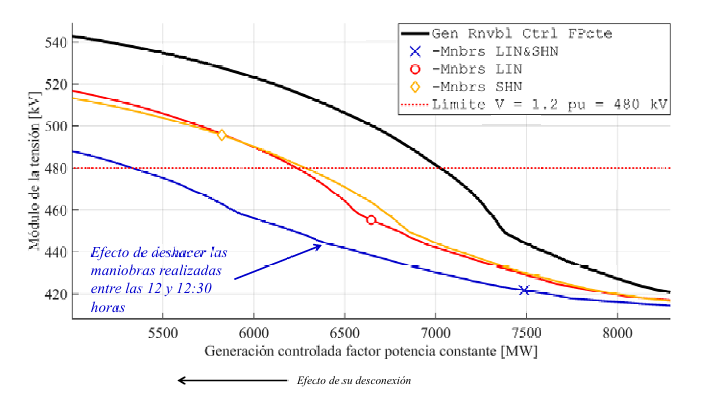
\includegraphics[width=0.85\textwidth]{figuras/fluctuaciones_tension_previas.png}
    \vspace{0.2cm}
    \caption[Curvas Q-V en Carmona 400 kV: efecto del mallado sobre el margen al colapso.]{%
    \textit{Curvas Q-V} de estabilidad de tensión en el nudo de
    Carmona~400~kV según el análisis pericial del IIT-ICAI.
    Fuente: Informe IIT-ICAI / Compass Lexecon \cite{icai2025}}
    \label{fig:curvas_qv_carmona}
\end{figure}
\vspace{0.6cm}

La figura~\ref{fig:curvas_qv_carmona} reproduce las \textit{Curvas
Q-V}\textsuperscript{\ref{anexo:curvas_qv}} en el nudo crítico de
Carmona~400~kV según el análisis del IIT-ICAI. Según dicho peritaje, las
maniobras de \textit{mallado} (LIN\&SHN) desplazaron el punto de
operación hacia la derecha, contrayendo el margen al colapso desde
2.964~MW hasta 1.268~MW. La línea discontinua roja marca el límite
$V = 1,2$~p.u. $= 480$~kV; la curva azul muestra que, según las
simulaciones del peritaje, revertir las maniobras habría preservado un
margen de seguridad sustancial.

La contracción en un 57\% del margen Q-V en Carmona llevó al sistema,
según el peritaje del IIT-ICAI, a un estado próximo al colapso: cualquier
perturbación posterior podía desencadenar un crecimiento incontrolado del
voltaje. La discrepancia entre las cifras de ICAI (2,4~GVAr) y el
análisis independiente del NREL (1,05~GVAr) no altera la conclusión
común entre ambos peritajes: en los dos casos, la inyección capacitiva
superó la capacidad de absorción residual del sistema \cite{icai2025}.

Bajo este marco de saturación capacitiva, el sector generador refuta la
calificación de ``disparos inadecuados'' emitida por REE, señalando una
limitación en la observabilidad del operador. Mientras el SCADA del
despacho central mostraba tensiones en la red de 400~kV dentro de los
límites normativos ---418~kV en el nudo de Granada en el instante del
disparo raíz---, el fenómeno del \textit{Tap-Lag} generaba, según el
peritaje, un punto ciego en las redes colectoras subyacentes. La
inercia mecánica de los \textit{Cambiadores de Tomas en Carga} (OLTC)
impidió que los transformadores ajustaran su relación de transformación
a tiempo, amplificando el transitorio hacia la red de 220~kV: el propio
titular de la infraestructura de Granada confirmó que la protección del
secundario detectó 244,32~kV ---más del 110~\% de la tensión nominal---
y que actuó correctamente. Para el peritaje del IIT-ICAI, los inversores
ejecutaron su protección conforme a la Orden TED/749/2020 y los Códigos
de Red RfG: los disparos no fueron un fallo de disciplina sino una
actuación normativa ante una condición impuesta por el propio sistema
\cite{icai2025,ree2025}.

La figura~\ref{fig:oscilografia_disparo_raiz} reproduce el registro
oscilográfico del disparo raíz aportado por el peritaje de IIT-ICAI.
El panel superior muestra la corriente trifásica ($I_A$, $I_B$, $I_C$),
estable en torno a 50~A hasta el disparo del interruptor aguas arriba
(\textit{Upstream breaker trip}), seguido de un transitorio de
cortocircuito y extinción. El panel inferior recoge la tensión en el
secundario de la red colectora ($U/\text{kV}$): la fase~A alcanza
aproximadamente 145~kV ($>$1,10~p.u.) en el instante del disparo. Según
la tesis pericial, este nivel resultó invisible para el SCADA de REE en
la red de 400~kV por el efecto del \textit{Tap-Lag}.

\vspace{0.6cm}
\begin{figure}[H]
    \centering
    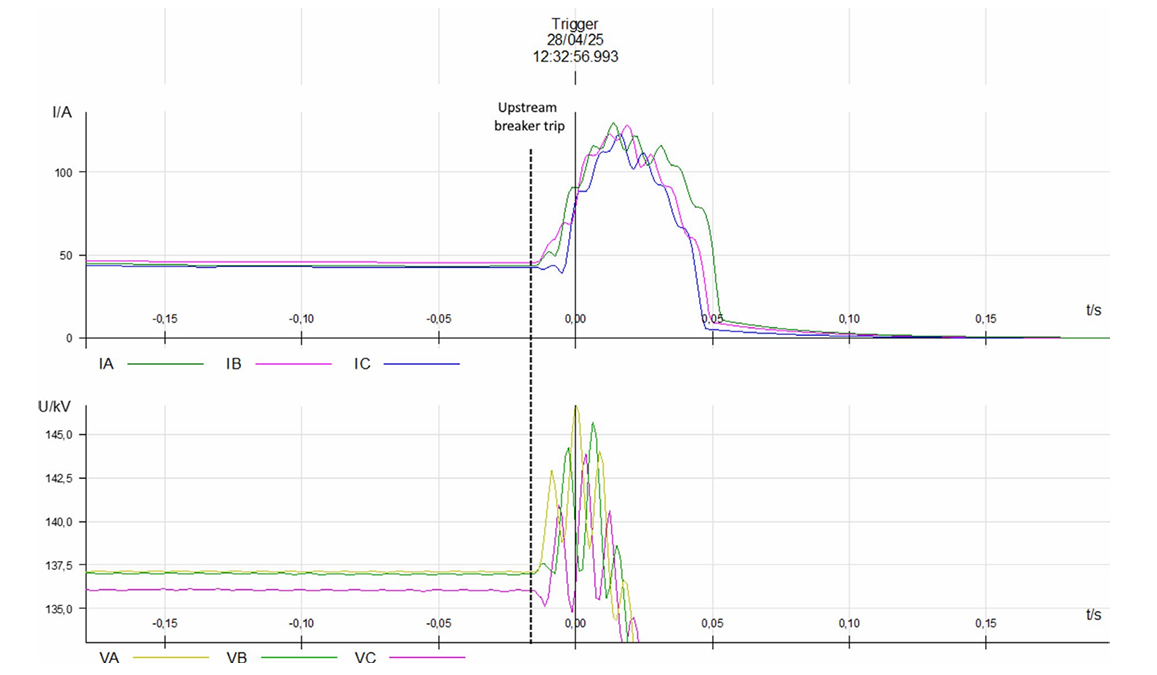
\includegraphics[width=0.85\textwidth]{figuras/aluvion_alertas_sobretension_sur.png}
    \vspace{0.2cm}
    \caption[Registro oscilográfico del disparo raíz en Granada (12:32:56.993 CEST).]{%
    Registro oscilográfico del disparo raíz a las 12:32:56.993~CEST en
    la subestación de Granada según el peritaje del IIT-ICAI.
    Fuente: Informe IIT-ICAI / AELEC \cite{icai2025}}
    \label{fig:oscilografia_disparo_raiz}
\end{figure}
\vspace{0.6cm}


La segunda línea argumental del informe pericial traslada la crítica
hacia la planificación del despacho y la rigidez regulatoria. El
P.O.~7.4, en su redacción anterior a la reforma, obligaba a la generación
del régimen RCR a operar con factor de potencia fijo, impidiendo que
los IBR utilizaran su electrónica de potencia para absorber o inyectar
potencia reactiva de forma dinámica, pese a disponer de esa capacidad
tecnológica. Según el peritaje, esta restricción excluía al 82~\% de la
generación instantánea del control activo de tensión, concentrando la
responsabilidad operativa en el escaso parque térmico síncrono
disponible \cite{icai2025}.

En ese contexto, el peritaje cuantifica la deficiencia más grave que
atribuye a la planificación del operador: en la zona sur ---epicentro
de las oscilaciones y del \textit{mallado}---, REE disponía de apenas
0,2~GVAr de capacidad de absorción de reactiva inductiva en la
generación convencional acoplada, frente a una inyección capacitiva
estimada superior a 0,7~GVAr derivada de las propias maniobras. El
desbalance era, según el informe del IIT-ICAI, matemáticamente
insalvable \cite{icai2025}.

\vspace{0.6cm}
\begin{figure}[H]
    \centering
    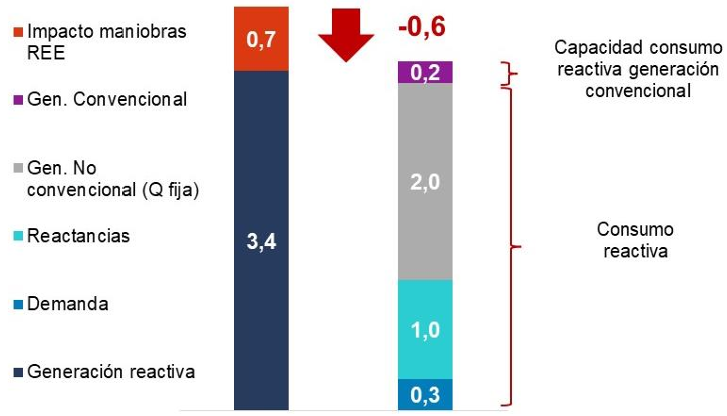
\includegraphics[width=0.65\textwidth]{figuras/asimetria_balance_reactiva_sur.png}
    \vspace{0.2cm}
    \caption[Balance de potencia reactiva: impacto de las maniobras de REE frente a la capacidad de absorción disponible.]{%
    Balance de potencia reactiva en el sistema, a las 12:30~CEST, según
    el análisis pericial del IIT-ICAI.
    Fuente: Informe IIT-ICAI / Compass Lexecon \cite{icai2025}}
    \label{fig:balance_reactiva_sistema}
\end{figure}
\vspace{0.6cm}

La figura~\ref{fig:balance_reactiva_sistema} desglosa el balance según
la lectura del peritaje. La barra izquierda recoge las fuentes de
generación de reactiva capacitiva: las maniobras de REE habrían aportado
0,7~GVAr adicionales sobre los 3,4~GVAr ya generados por las líneas. La
barra derecha muestra la capacidad de absorción disponible: la
generación convencional síncrona aportaba apenas 0,2~GVAr, insuficiente
---en la lectura del ICAI--- para compensar el exceso. El déficit neto
de $-0,6$~GVAr es presentado en el informe como expresión cuantitativa
del estrechamiento del margen Q-V que habría precedido a la cascada de
sobretensiones.

La conclusión del informe pericial es que el colapso resultó de la
convergencia de tres factores directamente atribuibles al operador y al
regulador: una maniobra de \textit{mallado} que ---en la lectura de
ICAI--- saturó los márgenes Q-V, una inobservabilidad estructural de la
red de 220~kV agravada por el \textit{Tap-Lag}, y un marco normativo
(P.O.~7.4) que impedía al 82~\% del parque generador participar en el
control dinámico de tensión \cite{icai2025}. Esta tesis es
diametralmente opuesta a la del Gobierno, que sitúa la causa en el
incumplimiento de los generadores; la resolución de esta contradicción
constituye el eje central del análisis comparativo de la
sección~\ref{sec:discrepancias}
(p.~\pageref{sec:discrepancias}).


% --------------------------------------------------------------
\section{La visión europea (Informe ENTSO-E): cumplimiento de los
\textit{Network Codes} RfG y separación del sistema síncrono}
\label{sec:vision_entsoe}
% --------------------------------------------------------------

Frente a la polarización del debate nacional, el panel de expertos de
ENTSO-E aporta una perspectiva factual centrada en la estabilidad del
área síncrona continental. Su informe de investigación cuestiona la
narrativa que atribuye el apagón a la penetración renovable \textit{per se}:
desde la óptica del panel europeo, el colapso del 28 de abril no se
debió a un exceso de generación renovable ni a una escasez inercial
primaria, sino a las limitaciones del marco vigente de control de
los perfiles de tensión del sistema. El incidente constituye un caso
de estudio europeo que evidencia la asimetría entre el despliegue
acelerado de activos renovable y la obsolescencia parcial de los
códigos de red que gobiernan su comportamiento dinámico
\cite{entsoe2025,mitceepr2025}.

El análisis de ENTSO-E identifica una tensión técnica fundamental: la
mayoría de las instalaciones fotovoltaicas y eólicas que se
desconectaron disponían de la electrónica de potencia necesaria para
realizar control de tensión robusto pero la normativa española vigente
les prohibía o no les exigía aportar este servicio dinámico,
forzándolas a operar con factores de potencia estáticos conforme al
RD~413/2014 \cite{gobierno2025,entsoe2025}. Esta restricción
regulatoria privó al sistema del soporte reactivo distribuido que
habría podido amortiguar la inyección capacitiva de las líneas en
vacío y constituye, para ENTSO-E, una de las vulnerabilidades
normativas centrales del incidente \cite{entsoe2025}.

\vspace{0.6cm}
\begin{table}[H]
\centering
\caption[Evolución de los requisitos para inversores IBR: NC RfG vigente vs NC RfG 2.0.]{%
Comparativa de los requisitos técnicos para módulos de generación no
síncrona según el \textit{Network Code on Requirements for
Generators}\textsuperscript{\ref{anexo:nc_rfg}} (NC~RfG) vigente y la
actualización NC~RfG~2.0 propuesta por ENTSO-E tras el incidente del
28 de abril. Fuente: Informe ENTSO-E \cite{entsoe2025}}
\label{tab:nc_rfg_comparativa}
\vspace{0.3cm}
\small
\begin{tabularx}{\textwidth}{>{\bfseries}p{3.8cm} >{\centering\arraybackslash}X >{\centering\arraybackslash}X}
\toprule
\textbf{Requisito} & \textbf{NC RfG vigente} & \textbf{NC RfG 2.0 (propuesto)} \\
\midrule
Modo de operación del inversor
    & \textit{Grid-following} (seguidor de red)
    & \textit{Grid-forming} (formador de red) obligatorio \\
\addlinespace
Umbral de aplicación
    & Varía por tipo de módulo y país
    & $\geq 1$~MW (PPM y ESM) \\
\addlinespace
Control de tensión
    & Factor de potencia fijo (estático)
    & Control dinámico continuo de $V$ y $Q$ \\
\addlinespace
Inercia
    & No requerida en IBR
    & \textit{Inercia sintética}\textsuperscript{\ref{anexo:inercia_sintetica}} obligatoria \\
\addlinespace
Capacidad \textit{Black Start}
    & No requerido en IBR
    & Capacidad de arranque en isla \\
\addlinespace
Referencia de sincronismo
    & Externa (PLL sobre red)
    & Generada internamente (fuente de tensión ideal) \\
\bottomrule
\end{tabularx}
\end{table}
\vspace{0.6cm}

La lección estructural que ENTSO-E extrae del cero de tensión es que el
paradigma de inversores en modo \textit{grid-following} (seguidor de
red)\textsuperscript{\ref{anexo:grid_forming}} resulta insuficiente, en
su opinión, para sistemas con alta penetración de IBR
\cite{entsoe2025,futured2024}. Como respuesta directa, la entidad ha
consolidado --en su Informe de Fase~II-- la actualización del NC~RfG~2.0, la cual prevé imponer el \textit{grid-forming} como requisito obligatorio
para todos los módulos de generación no síncrona y almacenamiento con
potencia igual o superior a 1~MW. Bajo este nuevo código, los
inversores deberán comportarse como fuentes de tensión ideales detrás
de una impedancia interna, garantizando el autosostenimiento de la red, la
aportación de inercia sintética y la supervivencia del equipo ante
perturbaciones severas de tensión, frecuencia y saltos de fase
\cite{entsoe2025,nrel2025}.

En lo relativo a la topología del incidente, ENTSO-E analiza la pérdida
de sincronismo y la separación del bloque ibérico como mecanismo de
protección del resto del continente. Durante la mañana del 28 de abril,
la interacción entre los generadores de la península y los del resto
del sistema europeo excitó oscilaciones inter-área en dos modos
diferenciados: una oscilación forzada de 0,6~Hz a las 12:03~CEST y un
modo natural Este-Centro-Oeste de 0,2~Hz a las 12:19~CEST, que
sometieron los corredores transfronterizos a un estrés electromecánico
significativo \cite{entsoe2025,nrel2025}. A las 12:33:19~CEST, cuando
la cascada de desconexiones por sobretensión barría internamente la
Península, la \textit{divergencia de polos} angular se volvió
insostenible y el sistema ibérico comenzó a perder la
\textit{estabilidad angular} con el área síncrona continental
\cite{entsoe2025}.

La figura~\ref{fig:perdida_sincronismo_frontera} reproduce la evolución
del intercambio en la frontera pirenaica durante la Fase~3. El panel
superior recoge el flujo neto total (INT\_FRA): el sistema pasó de
exportar 469~MW a las 12:32:57~CEST ---instante del disparo raíz en
Granada (línea naranja)--- a importar un máximo de $3.807$~MW a las
12:33:19,620~CEST, momento de la pérdida de sincronismo (línea
magenta). El panel inferior desglosa los flujos por circuito
(Vic-Baixas, Hernani, Arkale y LLG4ECSL). La oscilación de
importación-exportación que se aprecia en la fase final del registro
refleja el comportamiento dinámico de la divergencia de polos antes de
la apertura definitiva de los interruptores.

\vspace{0.6cm}
\begin{figure}[H]
    \centering
    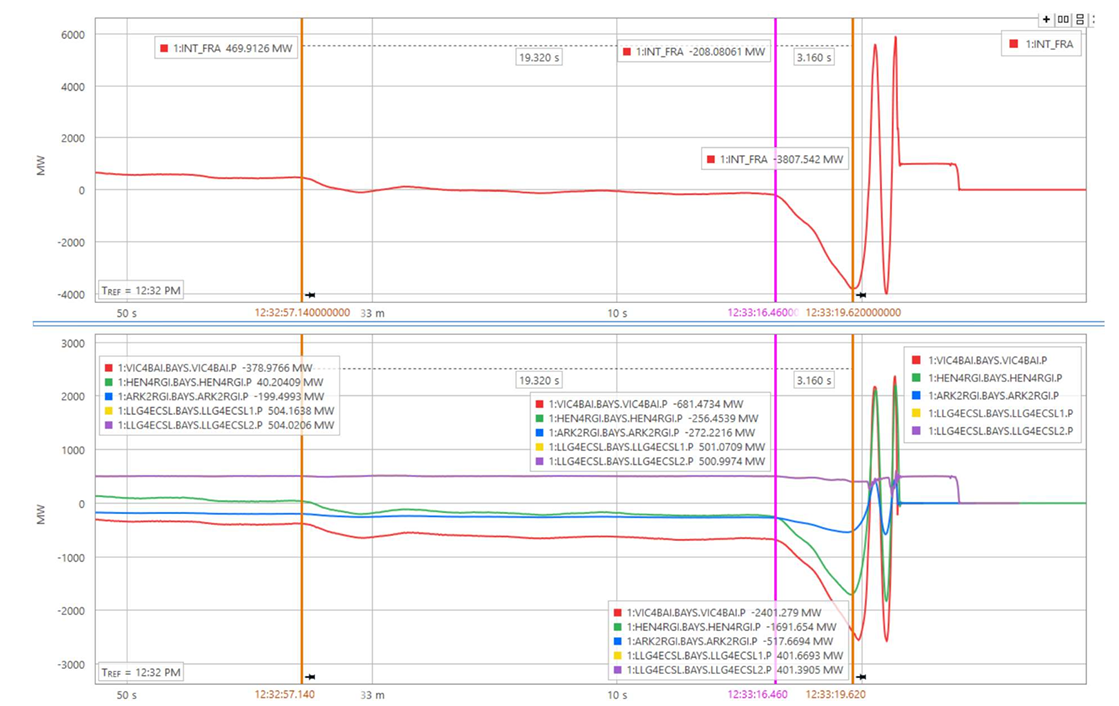
\includegraphics[width=0.95\textwidth]{figuras/perdida_sincronismo_frontera.png}
    \vspace{0.2cm}
    \caption[Evolución del intercambio España-Francia y pérdida de sincronismo (12:32:57--12:33:20 CEST).]{%
    Evolución del intercambio de potencia activa en la frontera
    España-Francia durante la Fase~3, según el Informe Factual de
    ENTSO-E.
    Fuente: Informe Factual ENTSO-E \cite{entsoe2025}}
    \label{fig:perdida_sincronismo_frontera}
\end{figure}
\vspace{0.6cm}


Ante la divergencia de polos, las \textit{protecciones de pérdida de
sincronismo} (\textit{Out-of-Step
Tripping}, OST)\textsuperscript{\ref{anexo:ost}} actuaron a las
12:33:21~CEST, ordenando la apertura automática de las líneas de
interconexión de corriente alterna a través de los Pirineos ---los
circuitos de 400~kV y 220~kV en Baixas-Vic, Argia-Arkale y
Argia-Hernani--- \cite{entsoe2025,ree2025}. Esta separación topológica
instantánea evitó que el colapso capacitivo y el hundimiento de la
frecuencia ---que alcanzó un RoCoF superior a 1,5~Hz/s--- arrastraran
al sistema francés y, por extensión, al resto de Europa Continental
\cite{entsoe2025}.

El informe de ENTSO-E concluye con una advertencia sobre la capacidad
de las herramientas de monitorización transfronteriza. Los análisis de
seguridad coordinada (CSA) y los modelos de red común (CGM), basados
en flujos de carga estáticos y en el Criterio $N-1$, evaluaron el
estado del sistema como ``Normal'' hasta los instantes previos al
colapso, como ya se analizó en la sección~\ref{sec:eas_entsoe}
(p.~\pageref{sec:eas_entsoe}). Para ENTSO-E, esta limitación frente a
dinámicas ultrarrápidas de sobretensión en redes de baja inercia
indica que los estándares de evaluación de la seguridad operativa
continental, diseñados para el comportamiento de máquinas síncronas
convencionales, resultan estructuralmente insuficientes para prevenir
colapsos en sistemas con alta penetración de electrónica de potencia
\cite{entsoe2025,mitceepr2025,blackswan2025}.

% --------------------------------------------------------------
\section{Discrepancias y consenso: comparativa técnica de los argumentos de los agentes}
\label{sec:discrepancias}
% --------------------------------------------------------------

El escrutinio cruzado de los dictámenes oficiales e independientes
constituye el núcleo analítico de este trabajo. La confrontación
técnica pivota sobre una dicotomía fundamental: determinar si el cero
de tensión fue la consecuencia de un error operativo sistémico del
despacho central o el resultado de un fallo generalizado en el
comportamiento técnico de los generadores privados ante una
perturbación externa. La Tabla~\ref{tab:consenso}
(p.~\pageref{tab:consenso}) recoge los puntos de acuerdo verificados
entre las cuatro fuentes y la Tabla~\ref{tab:discrepancias}
(p.~\pageref{tab:discrepancias}) organiza las divergencias
irreconciliables \cite{gobierno2025,ree2025,icai2025,entsoe2025}.

\clearpage
% ============================================================
\subsection*{Puntos de consenso técnico entre los cuatro informes}
% ============================================================

A pesar de la polarización del debate, existe un conjunto de
conclusiones técnicas sobre las que todos los informes convergen, cuya
importancia radica precisamente en que matizan o desmienten algunas
de las narrativas mediáticas más extendidas.

\begin{table}[H]
\centering
\caption[Puntos de consenso técnico entre los cuatro informes oficiales e independientes.]{Puntos de consenso técnico entre los cuatro informes oficiales e independientes. Fuente: Elaboración propia}
\label{tab:consenso}
\vspace{0.3cm}
\small
\begin{threeparttable}
\begin{tabularx}{\textwidth}{>{\bfseries}p{3.6cm} X >{\centering\arraybackslash}p{0.65cm}
>{\centering\arraybackslash}p{0.65cm} >{\centering\arraybackslash}p{0.85cm}
>{\centering\arraybackslash}p{1cm}}
\toprule
\textbf{Punto de consenso} & \textbf{Fundamento técnico compartido}
& \textbf{GOB} & \textbf{REE} & \textbf{ICAI} & {\textbf{ENT-E}} \\
\midrule

La inercia no fue la causa raíz &
El sistema operaba con $H = 2,3$~s, por encima del umbral de 2,0~s
recomendado por ENTSO-E. Una mayor inercia habría ralentizado la caída
de frecuencia décimas de segundo, sin evitar el colapso por
sobretensión.
& \checkmark & \checkmark & \checkmark & \checkmark \\
\addlinespace

Colapso por sobretensión, no por déficit de frecuencia &
La causa material del apagón fue la inestabilidad capacitiva
(desequilibrio de potencia reactiva $Q$) que provocó disparos por sobretensión en
cascada, no una pérdida de potencia activa $P$ ni una
caída de frecuencia primaria.
& \checkmark & \checkmark & \checkmark & \checkmark \\
\addlinespace

Las reservas de potencia activa eran suficientes &
En el momento del incidente, la reserva terciaria a subir superaba
los 7.000~MW, descartando una crisis de capacidad de generación como
factor causante.
& \checkmark & \checkmark & \checkmark & \checkmark \\
\addlinespace

El UFLS agravó el colapso de tensión &
El deslastre automático de cargas, al eliminar los últimos sumideros
de reactiva inductiva (motores e industria), aceleró la escalada de
tensión que ya estaba destruyendo la red. Las lógicas de defensa
diseñadas para déficit de frecuencia resultaron contraproducentes
ante un colapso capacitivo.
& \checkmark & \checkmark & \checkmark & \checkmark \\
\addlinespace

Las protecciones de sincronismo actuaron correctamente &
La apertura de los circuitos transpirenaicos a las 12:33:21~CEST
(Baixas-Vic, Argia-Arkale, Argia-Hernani) fue técnica y normativamente
correcta: impidió el contagio del colapso al sistema europeo
continental.
& \checkmark & \checkmark & \checkmark & \checkmark \\
\addlinespace

La normativa IBR era insuficiente &
El P.O.~7.4 y el RD~413/2014 impedían a los IBR participar en el
control dinámico de tensión pese a disponer de capacidad tecnológica
para ello. Esta restricción regulatoria privó al sistema del soporte
reactivo distribuido más abundante.
& \checkmark & \checkmark & \checkmark & \checkmark \\
\addlinespace

El Criterio $N-1$ estático es insuficiente &
Las herramientas de seguridad basadas en flujos de carga estáticos
(análisis $N-1$) evaluaron el sistema como seguro horas antes del
colapso, sin capacidad para anticipar la dinámica ultrarrápida de
inestabilidad capacitiva característica de redes de baja inercia.
& \checkmark & \checkmark & \checkmark & \checkmark \\

\bottomrule
\end{tabularx}
\begin{tablenotes}
\footnotesize
\item GOB = Comité de Análisis del Gobierno;
REE = Red Eléctrica de España;
ICAI = IIT-ICAI / Compass Lexecon / AELEC;
ENT-E = Panel de Expertos ICS.
\end{tablenotes}
\end{threeparttable}
\end{table}
\clearpage

% ============================================================
\subsection*{Divergencias técnicas irreconciliables}
% ============================================================

Los puntos de consenso anteriores delimitan el terreno común; lo que
sigue es la fractura. La Tabla~\ref{tab:discrepancias}
(p.~\pageref{tab:discrepancias}) sistematiza los cinco ejes de disputa
en los que las posiciones de los informes son directamente
contradictorias. La resolución de estas contradicciones tiene
implicaciones jurídicas y regulatorias directas, puesto que determina
si la responsabilidad recae sobre el operador, sobre los generadores
o sobre el marco normativo.

\begin{landscape}
\begin{table}[H]
\centering
\caption[Divergencias técnicas irreconciliables entre los informes sobre el apagón del 28 de abril.]{%
Sistematización de los cinco ejes de disputa técnica entre los
informes analizados. $\bullet$ = posición principal adoptada por el
informe; $\circ$ = posición intermedia o parcialmente compartida.
GOB/REE = Comité de Análisis del Gobierno e Informe de Red Eléctrica;
ICAI = IIT-ICAI / Compass Lexecon / AELEC; ENTSO-E = Panel de Expertos
ICS. Fuente: Elaboración propia}
\label{tab:discrepancias}
\vspace{0.3cm}
\footnotesize
\setlength{\tabcolsep}{6pt}
\begin{tabular}{p{3.2cm} p{6.5cm} p{6.5cm} p{5.5cm}}
\toprule
\textbf{Eje de disputa}
& \textbf{Gobierno / REE}
& \textbf{ICAI / AELEC}
& \textbf{ENTSO-E} \\
\midrule

\textbf{1. Origen de la saturación capacitiva}
&
$\bullet$ El sistema tenía márgenes suficientes. La saturación se
produjo porque los generadores no absorbieron la potencia reactiva
requerida (P.O.~7.4 y RD~413/2014). El \textit{mallado} fue una medida
protocolizada y necesaria ante las oscilaciones.
&
$\bullet$ El \textit{mallado} de 11 líneas en vacío inyectó
1,05--2,4~GVAr capacitivos por \textit{Efecto Ferranti}, contrayendo
el margen Q-V de Carmona en un 57~\% ($2.964 \to 1.268$~MW). El colapso
era matemáticamente inevitable antes de que fallara ninguna planta.
&
$\circ$ No atribuye causalidad al \textit{mallado} pero documenta
que los RCC no detectaron la saturación capacitiva. Identifica la
restricción normativa de los IBR como la vulnerabilidad estructural
primaria. \\
\addlinespace\midrule

\textbf{2. Naturaleza de la oscilación de 0,6~Hz}
&
$\bullet$ Oscilación forzada con origen en el lazo de control de una
planta fotovoltaica en Badajoz. Este comportamiento anómalo es el
detonante de la secuencia de eventos que llevó al colapso.
&
$\bullet$ Las evidencias no son concluyentes. La oscilación pudo ser
un modo inter-área natural amplificado por el ratio de amortiguamiento
próximo al 1~\%, consecuencia de la ausencia de
\textit{Estabilizadores del Sistema de
Potencia}\textsuperscript{\ref{anexo:pss}} (PSS) activos en los ciclos
combinados apagados en la zona sur.
&
$\circ$ Documenta la oscilación como atípica (0,6~Hz, detectada hasta
Alemania) pero no atribuye causalidad definitiva. Señala que la baja
inercia amplificó cualquier perturbación de origen. \\
\addlinespace\midrule

\textbf{3. Legitimidad de los disparos en cascada (\textit{Tap-Lag})}
&
$\bullet$ Los primeros disparos (12:32:57--12:33:18~CEST) fueron
``inadecuados'' o prematuros: el SCADA de REE registraba 418~kV en la
red de 400~kV, dentro de los límites del P.O.~1.1 ($\leq 435$~kV).
&
$\bullet$ Los disparos fueron normativamente correctos. El
\textit{Tap-Lag} creó un punto ciego: las redes colectoras de 220~kV
alcanzaban 244~kV ($>$1,10~p.u.), invisibles para el SCADA. El titular
de la ICE de Granada confirmó que su protección actuó correctamente.
&
$\circ$ No califica los disparos como inadecuados. Subraya la
inobservabilidad de la red subyacente como limitación sistémica del
operador y de los RCC. \\
\addlinespace\midrule

\textbf{4. Despacho en la zona sur}
&
$\circ$ Reconoce la indisponibilidad del ciclo combinado andaluz
desde la tarde del 27 de abril. Justifica la no sustitución por los
niveles de tensión adecuados en ese momento y la disponibilidad de
otros recursos en la región.
&
$\bullet$ La zona sur disponía de solo 0,2~GVAr de absorción frente a
$>$0,7~GVAr de inyección capacitiva inducida por el propio operador.
La no sustitución del ciclo combinado fue la decisión de despacho
más determinante del incidente.
&
$\circ$ No se pronuncia sobre la decisión individual de despacho
pero señala la baja potencia de cortocircuito en Andalucía como
factor estructural agravante. \\
\addlinespace\midrule

\textbf{5. Responsabilidad principal}
&
$\bullet$ Los generadores incumplieron sus obligaciones de control de
tensión. Si todos los agentes hubieran cumplido la normativa vigente
en su punto de conexión, el sistema habría absorbido el transitorio.
El apagón fue un fallo del parque generador privado.
&
$\bullet$ REE llevó la red a un estado de colapso inevitable mediante
el \textit{mallado}, con visibilidad insuficiente y despacho
inadecuado. Los generadores actuaron conforme a la física y a la
normativa en su punto de conexión. El apagón fue un fallo del
operador y del regulador.
&
$\bullet$ La causa raíz es normativa: la restricción regulatoria que
impedía a los IBR controlar tensión dinámicamente. El fallo es del
sistema regulatorio europeo y nacional, no atribuible exclusivamente
a ningún agente. \\

\bottomrule
\end{tabular}
\end{table}
\end{landscape}

% ============================================================
\subsection*{Síntesis interpretativa}
% ============================================================

La comparativa técnica de este trabajo permite trascender la disputa
entre partes y formular un diagnóstico de segundo orden: el apagón
del 28 de abril de 2025 no fue ni un ``Cisne Negro'' imprevisible
ni el fracaso de una tecnología concreta, sino la manifestación
convergente de tres fracturas de gobernanza que coexistían en el
sistema eléctrico ibérico
\cite{gobierno2025,icai2025,entsoe2025,mitceepr2025,blackswan2025}.

\subsubsection*{Fractura operativa: causalidad frente a responsabilidad}

El debate nuclear entre REE e ICAI es, en última instancia, una
disputa sobre el primer eslabón de la cadena causal. La tesis del
\textit{mallado} como detonante (ICAI) y la tesis del incumplimiento
colectivo como causa (REE / Gobierno) no son mutuamente excluyentes
en términos técnicos: ambos factores contribuyeron a la
saturación capacitiva que estrechó los márgenes Q-V. Lo que sí son
excluyentes es su implicación jurídica y económica pues determinan
sobre quién recae la responsabilidad material del colapso. Esta
ambigüedad causal no es un accidente analítico; es el resultado
previsible de operar una red sin instrumentación dinámica suficiente:
cuando el sistema no dispone de PMU en todos los nudos críticos ni
de herramientas de cálculo de estabilidad de tensión en tiempo real,
la reconstrucción forense posterior queda inevitablemente sujeta a
interpretación. El consenso tácito entre las partes ---que ningún
informe enuncia explícitamente--- es que la arquitectura de
monitorización del sistema resultó insuficiente para haber gestionado
el incidente en tiempo real o para resolverlo unívocamente a
posteriori \cite{ree2025,icai2025,entsoe2025}.

\subsubsection*{Fractura regulatoria: una normativa del siglo XX
aplicada a una red del siglo XXI}

La posición de ENTSO-E ---la más estructural de las tres--- apunta a
que tanto el operador como los generadores actuaron dentro de los
límites de una normativa que era inadecuada para el sistema que
pretendía gobernar \cite{entsoe2025}. El P.O.~7.4 y el RD~413/2014
diseñaron un esquema de control de tensión para una red dominada por
masas síncronas de respuesta lenta; aplicarlo a una red con 82~\% de
penetración IBR equivale, en términos de ingeniería de control, a
intentar estabilizar un sistema de respuesta en milisegundos con un
regulador diseñado para dinámicas de minutos
\cite{entsoe2025,futured2024,nrel2025}. Esta inadecuación no era
desconocida: la propuesta de actualización del P.O.~7.4 llevaba años
en proceso de aprobación regulatoria y el propio informe del
Gobierno reconoce que su entrada en vigor habría sido el cambio más
relevante para haber evitado el colapso \cite{gobierno2025}. El
apagón del 28 de abril es, en este sentido, el coste medible de una
demora regulatoria \cite{mitceepr2025}.

\subsubsection*{Fractura sistémica: herramientas de seguridad
estáticas en una red dinámica}

El consenso unánime sobre la insuficiencia del Criterio $N-1$
estático apunta a una vulnerabilidad que trasciende ampliamente el
caso ibérico \cite{entsoe2025,nrel2025,mitceepr2025}. Los modelos de
flujo de carga que evaluaron el sistema como ``Normal'' horas antes
del colapso son matemáticamente incapaces de representar fenómenos
de inestabilidad capacitiva en redes de baja inercia: no resuelven
ecuaciones diferenciales, no modelan la dinámica de los lazos de
control de los inversores y no calculan márgenes Q-V en tiempo
real \cite{entsoe2025}. Esta limitación no es un fallo puntual de
los operadores del 28 de abril; es la condición habitual de
operación de todos los despachos europeos. La velocidad a la que
progresó el colapso ---de los primeros disparos al cero de tensión
en menos de 90 segundos--- sitúa el fenómeno fuera del horizonte
temporal de cualquier intervención humana: cuando el operador
percibió la gravedad del transitorio, el sistema ya era
irrecuperable \cite{ree2025,entsoe2025}. La única respuesta viable
a esta escala temporal es la prevención estructural mediante
herramientas de análisis de seguridad dinámica en tiempo real, cuyo
despliegue en los centros de coordinación regional europeos
constituye una de las reformas más urgentes identificadas por
ENTSO-E \cite{entsoe2025,mitceepr2025}.

\subsubsection*{Implicación de fondo: el límite del paradigma
centralizado}

Subyacente a las tres fracturas anteriores existe una tensión más
profunda que los informes abordan de forma fragmentaria pero que
este análisis comparativo permite formular con claridad: el
paradigma de operación centralizada ---un operador único con
visibilidad limitada al nivel de 400~kV, que despacha generación
síncrona mediante señales de mercado horarias y gestiona la tensión
con reactancias de conmutación discreta--- fue diseñado para una red
en la que la masa síncrona proporcionaba amortiguamiento natural y
los generadores respondían en segundos a las consignas del despacho
\cite{futured2024,nrel2025}. En una red donde el 82~\% de la
generación está formada por inversores que responden en
milisegundos, se autoproveen de referencias de sincronismo mediante
PLL, y cuyo comportamiento dinámico es opaco para el SCADA de
400~kV, ese paradigma ha alcanzado los límites de su capacidad de
gestión \cite{entsoe2025,nrel2025,futured2024}. El 28 de abril de
2025 no es, por tanto, únicamente el caso de estudio de un apagón:
es el evento que señala el agotamiento del modelo de despacho
centralizado en sistemas con alta penetración de electrónica de
potencia y el punto de partida obligatorio de una nueva
arquitectura de control distribuido y en tiempo real para la red
europea del siglo XXI \cite{entsoe2025,mitceepr2025,blackswan2025}.